\chapter{Physikalischer Hintergrund}
%
\section{Das Standardmodell der Teilchenphysik}
%
Das Standardmodell (SM) der Teilchenphysik beschreibt den Aufbau der Materie, sowie ihre Wechselwirkung auf elementarer Ebene. Sie stellt eine über viele Jahrzehnte auf der speziellen Relativitätstheorie sowie der Quantentheorie erwachsene und vielfältig getestete Theorie dar. Allgemein werden zunächst zwei Arten von Teilchen unterschieden: Fermionen (halbzahliger Spin $s=\sfrac{\hbar}{2}$)($\hbar$: reduziertes Plancksches Wirkungsquantum) und Bosonen (ganzzaliger Spin $s=\hbar$). Die Fermionen nach dem Standardmodell sind in drei Generationen von Quarks, sowie drei Generationen von Leptonen unterteilt, wie sie unten aufgeführt sind. Die Leptonengenerationen bestehen hierbei aus einem ganzzahlig (in Einheiten der Elementarladung) geladenen punktförmigen Lepton ($e$, $\mu$, $\tau$), sowie den dazugehörigen ungeladenen und masselosen Neutrinos $\nu_e$, $\nu_\mu$, $\nu_\tau$.
%
\begin{figure}
  \centering
      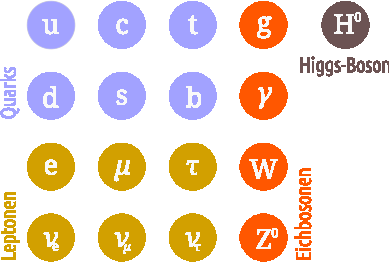
\includegraphics[width=0.6\textwidth]{Plots/SM.pdf}
  \caption{Die Elementarteilchen im Stadardmodell der Teilchenphysik.}
  \label{fig:particles}
\end{figure}
%
Auch die Quarks gliedern sich in drei Generationen. Diese erfolgt über die Eigenschaften der Teilchen: die Quarks lassen sich in \textit{up-artige} Quarks mit Ladung $\sfrac{2}{3}$, sowie \textit{down-artige} mit Ladung $\sfrac{-1}{3}$ einteilen. Es gilt für diese Darstellung dass die Teilchenmassen zwischen den Generationen von links nach rechts zunehmen.\\
Im Standardmodell unterscheidet man zwischen drei Wechselwirkungen der Elementarteilchen untereinander: die starke Wechselwrikung zwischen farbgeladenen Teilchen, die schwache Wechselwirkung an welcher alle Elementarteilchen teilnehmen, sowie die elektromagetische Wechselwirkung, welcher nur elektrisch geladene Teilchen unterliegen. Die letzten beiden lassen sich im Rahmen des SM zur elektroschwachen Wechselwirkung vereinigen.
Die Farbladung in der starken Wechselwirkung beschreibt das Konzept einer Quantenzahl deren Existenz zur theoretischen Umsetzung des sogenannten \textit{confinement} dient. \textit{confinement} meint hierbei die Tatsache, dass alle elementaren Teilnehmer der starken Wechselwirkung nur in "farbneutralen" (z.B. Farbe + Antifarbe) Zuständen frei existieren; freie Quarks lassen sich, da sie eine von null verschiedene Farbladung tragen also nicht beobachten.\\
%
Die Übertragung der Wechselwirkungen findet über die oben genannten Bosonen statt. Bei der starken Wechselwirkung sind dies die acht verschiedenen Gluonen ($g$). Sie tragen eine Farbladung und einen ganzzahligen Spin $\hbar$. Die Austauschteilchen der elektroschwachen Wechselwirkung sind die Photonen ($\gamma$) für den elektromagnetischen Teil, sowie für die schwache Wechselwirkung das neutrale $\symup{Z}$-Boson und die geladenen $\symup{W^{\pm}}$-Bosonen. \\
%
Aus den oben aufgeführten Quarks existieren über Kombination mehrere so genannte Hadronen - also über Resonanz aus Quarks zusammengesetzte Teilchen. Hierbei unterscheidet man die aus Quark und Antiquark bestehenden Mesonen und die aus drei Quarks (Antiquarks) bestehenden Baryonen. Zu den Mesonen zählt beispielsweise auch das $J/\!\symup{\Psi}$ mit einem Quarkinhalt von $(c\bar{c})$, während das Proton ein prominenter Vertreter der Baryonen ist. Die meisten der aus den sechs Quarks sowie deren Antiteilchen gebildeten Hadronen sind nicht stabil, sodass sie über eine der oben genannten Wechselwirkungen in andere Hadronen zerfallen. Ähnliches lässt sich auch durch Streuprozesse oder Kollisionen erzielen, wie sie beispielsweise am LHC stattfinden.\\
%
Im Standardmodell sind bei all solchen Zerfällen diverse Erhaltungsgrößen zu beachten. Neben den klassischen Größen, wie etwa Energie- oder Impulserhaltung sind für die verschiedenen Wechselwirkungen auch einige Quantenzahlen im Teilchenzerfall invariant. Eines der fundamentalen Konzepte ist die \textit{lepton-flavor}-Erhaltung.
%
\section{\texorpdfstring{LFV und der Zerfall $\symup{J}/\symup{\Psi}\rightarrow e^{\pm}\mu^{\mp}$}{Jpsi to eµ}}
%
Wie in der Einleitung bereits erwähnt, ist der Signalzerfall \signal ein im Standardmodell verbotener Zerfall, weil er die Erhaltung des \textit{lepton-flavor} verletzt. Jedem Lepton wird hierbei gemäß der in Abbildung~\ref{fig:particles} aufgeführten Generationen eine Quantenzahl zugeordnet (der \textit{lepton-flavor}). Elektronen oder Elektronneutrinos besitzen beispielsweise die Quantenzahl $l_e=1$, aber $l_\mu=0$, während Myonen $l_\mu=1$ und $l_e=0$ tragen. Antiteilchen wird jeweils der Wert $-1$ zugeordnet. So lassen sich Teilchenzerfälle auf die Erhaltung des \textit{lepton-flavor} überprüfen; der Zerfall \signal verstößt hierbei offensichtlich gegen diese Erhaltung.\\
%
Es gibt einige theoretische Vorhersagen über Mechanismen und Möglichkeiten der LFV; die meisten davon beschreiben Physik jenseits des Standardmodells. Ein im Standardmodell über Neutrinooszillation möglicher Zerfall ist in der folgenden Abbildung dargestellt.
%
\begin{figure}[H]
  \centering
  \begin{tikzpicture}
    \tikzfeynmanset{ every vertex={ black, dot}}
    \begin{feynman}
      \vertex (a1) {\(\mu\)};
      \vertex[right=1cm of a1] (a2);
      \vertex[right=2cm of a2] (a3);
      \vertex[right=1cm of a3] (a4) {\(e\)};
      \vertex at ($(a2)!1cm!(a3)!0.75!90:(a3)$) (d);
      \vertex[above=1.5cm of a4] (c){\(\gamma\)};
      \diagram*{
        (a1) -- [fermion](a2),
        %(a2) -- [fermion](a3),
        %(a2) -- [plain, edge label'=\(\nu_\mu\), insertion={0.5}] (a3),
        (a2) -- [fermion, edge label'=\(\nu_\mu/\nu_e\)](a3),
        (a2) -- [boson, quarter left, edge label=\(W\)] (d) [square dot] -- [boson,quarter left, edge label=\(W\)] (a3),
        (a3) -- [fermion](a4),
        (d) --  [photon, quarter left](c)
          };
    \end{feynman}
  \end{tikzpicture}
  \label{fig:lfv_nu}
\end{figure}
%
Da die Masse der Neutrinos nicht verschwindend ist, können so gennante Oszillationen in andere \textit{flavors} stattfinden. Über diesen Mechanismus ist ein Zerfall möglich der an jedem Vertex \textit{lepton-flavor}-erhaltend ist. Da die Massen der Neutrinos allerdings als sehr klein abgeschätzt werden können, sind die Beiträge dieses Zerfallskanals zu gering, als dass sie experimentell nachgewiesen werden können. Experimentelle Evidenz deutete daher auf Physik jenseits des Stadardmodells hin. Andere theoretische Beschreibungen gehen etwa von Zerfällen über ein $Z'$-Boson aus.\cite{zprime} Auch Prozesse über SUSY Teilchen sind nicht ausgeschlossen\cite{susy_gut1}\cite{susy_gut2}.
